% Created 2020-04-24 vie 23:03
% Intended LaTeX compiler: pdflatex
\documentclass[11pt,a4paper]{article}
\usepackage[utf8]{inputenc}
\usepackage[T1]{fontenc}
\usepackage{graphicx}
\usepackage{grffile}
\usepackage{longtable}
\usepackage{wrapfig}
\usepackage{rotating}
\usepackage[normalem]{ulem}
\usepackage{amsmath}
\usepackage{textcomp}
\usepackage{amssymb}
\usepackage{capt-of}
\usepackage{hyperref}
\usepackage{tabularx}
\usepackage{lastpage}
\usepackage{enumitem}
\usepackage[english, spanish]{babel}
\usepackage[table,xcdraw]{xcolor}
\usepackage[left=2.00cm, right=2.50cm, top=2.50cm, bottom=2.50cm]{geometry}


\newcommand*{\autor}[1]{\def\authorname{#1}}
\newcommand*{\titulo}[1]{\def\@title{#1}\def\ttitle{#1}}

\renewcommand{\contentsname}{Índice}
\newcommand{\versionActual}{A}
\newcommand{\fechaA}{07/07/2025}
\newcommand{\fechaB}{}
\newcommand{\fechaC}{}

\newcommand{\docCode}{\normalsize RETRO\_GAME-RS versión \versionActual}

\usepackage{ifthen}
\newcommand{\fechaActual}{%
  \ifthenelse{\equal{\versionActual}{A}}{\fechaA}{%
    \ifthenelse{\equal{\versionActual}{B}}{\fechaB}{%
      \ifthenelse{\equal{\versionActual}{C}}{\fechaC}{
        N/A
      }}}}

\titulo{Videojuego portátil inspirado en consolas retro} 
\autor{Lic. Jezabel Danon}

\usepackage{fancyhdr}
\fancyhf{} % clear all header and footers
\pagestyle{fancy}
\lhead{
\includegraphics[width=3.5cm]{../Figuras/logoFIUBA.pdf}}
\chead{}
\rhead{\normalsize \textrm{ \textbf{\@title} \\ Especificación de requerimientos de software \\ \docCode}}
\setlength{\footskip}{25pt}
\lfoot{ }
\cfoot{\normalsize Página \thepage \hspace{1px} de \pageref{LastPage}}
\rfoot{}
\setlength{\fboxrule}{4pt} \setlength{\fboxsep}{2ex}
\setlength{\headheight}{42pt}

\renewcommand{\headrulewidth}{1.0pt}
\renewcommand{\footrulewidth}{0.4pt}

\hypersetup{
   colorlinks=true,
  linkcolor=black,      % color para enlaces internos (índice, referencias)
  citecolor=black,      % color para citas (si usás biblatex)
  filecolor=black,      % enlaces a archivos
  urlcolor=blue,        % color para \href y \url
 pdftitle = {\@title},
 pdfauthor = {\authorname},
 pdfkeywords={},
 pdfsubject={},
%  pdfcreator={Emacs 26.2 (Org mode 9.1.9)}, 
 pdflang={es}
}


% \renewcommand{\thesection}{\arabic{section}.}
% \renewcommand{\thesubsection}{\thesection\arabic{subsection}.}
% \renewcommand{\thesubsubsection}{\thesubsection\arabic{subsubsection}.}

%  COMIENZA EL DOCUMENTO --------------------------------------------------------------------
\begin{document}

% \maketitle
\begin{titlepage}
    \centering

    
\includegraphics[width=.7\textwidth]{../Figuras/logoFIUBA.pdf}\par
    \vspace{1cm}

    
    \vspace{3cm}
    {\Huge \textbf{\ttitle}} \\
    \vspace{2cm}

    {\Large\itshape Especificación de requerimientos de software\par}
    \vspace{4cm}

    
    
    \flushleft
    {\normalsize Autor:\\}
    {\Large \authorname \ (jezabel.danon@gmail.com)\\}
    \vspace{1.5cm}

    {\scshape\LARGE \fechaActual \par} 
    {\scshape\LARGE Versión \versionActual \par}

    \vfill
    \centering
    \textit{Este documento fue creado en base al estándar IEEE-830 durante el curso de Ingeniería de Software entre el 26 de junio de 2025 y el 21 de agosto de 2025.}
\end{titlepage}

\clearpage            % fuerza una nueva página real
\pagestyle{fancy}     % activa encabezado y pie desde esta página

\section*{Historial de cambios}
\pagestyle{fancy}     % activa el estilo fancy para el resto
\begin{table}[ht]
\label{tab:registro}
\centering
\begin{tabularx}{\linewidth}{@{}|c|c|X|c|c|@{}}
\hline
\rowcolor[HTML]{C0C0C0} 
Versión & Fecha & \multicolumn{1}{c|}{\cellcolor[HTML]{C0C0C0}Descripción}  & Autor & Revisores     \\ \hline
A   & \fechaA   & Creación del documento     & \authorname     &                        \\ \hline
% 1      & Se completa hasta el punto 5 inclusive                & {10} de {mayo} de 2025 \\ \hline
% 2      & Se completa hasta el punto 9 inclusive \newline
% 		  Agrega usuario final \newline
% 		  Cambio de cliente \newline
% 		  Cambio de título del proyecto                    & {19} de {mayo} de 2025 \\ \hline
% 3      & Se completa hasta el punto 12 inclusive\newline
% 		  Modificación del formato de las historias de usuario \newline
% 		  Reducción de horas del proyecto 					& {27} de {mayo} de 2025 \\ \hline
% 4      & Se completa el plan \newline
% 		  Se agrega el nombre del director \newline
% 		  Corrección de errores	                                 & {3} de {junio} de 2025 \\ \hline
% 5      & Corrección del punto 14                          & {6} de {junio} de 2025 \\ \hline

\end{tabularx}
\end{table}

\pagebreak

\tableofcontents

\pagebreak

\section{Introducción}
\label{sec:org60390fa}

\subsection{Propósito}
\label{sec:org434c3ef}
\begin{enumerate}
  \item Este documento representa una especificación de requerimientos de software para el sistema embebido \textit{\ttitle}. 
  \item Está dirigido a los desarrolladores que se ocupen del análisis, diseño e implementación del software, así como también a quienes desarrollen el testing, validaciones y/o verificaciones del mismo.
\end{enumerate}


\subsection{Ámbito del sistema}
\label{sec:org12e44a1}

\begin{enumerate}
  \item El software a desarrollar controlará la interfaz de usuario de la consola de juegos y procesará las entradas y salidas de los periféricos. 
  \item Las entradas del sistema serán:
  \begin{itemize}
    \item Botones
    \item Joystick analógico
    \item Acelerómetro
  \end{itemize}
  \item Las salidas del sistema serán:
  \begin{itemize}
    \item Pantalla
    \item Salida de audio
    \item Motor de vibraciones
  \end{itemize}
\end{enumerate}


\subsection{Definiciones, Acrónimos y Abreviaturas}
\label{sec:orgb158e36}

\begin{enumerate}
  \item Acrónimos:
  \begin{itemize}
    \item IEEE: Instituto de Ingenieros Eléctricos y Electrónicos.
    \item ERS: Especificación de Requisitos de Software.
    \item RTOS: Sistema Operativo de Tiempo Real (Real Time Operating System).
    \item CMSIS: Arm's Common Microcontroller Software Interface Standard. Se compone por un conjunto de APIS, componentes de software, herramientas y flujos de trabajo provisto por el desarrollador de la arquitectura del microcontrolador a utilizar.
    \item HAL: Hardware Abstraction Layer. Conjunto de bibliotecas de software provistas por STMicroelectronics para simplificar la interacción con el hardware de microcontroladores STM32.
    \item UI: Interfaz de usuario (User Interface).
    \item UART: Universal Asynchronous Receiver/Transmitter. 
    \item I2C: Inter-Integrated Circuit.
    \item SPI: Serial Peripheral Interface.
    \item ADC: Analogic to Digital Converter.
    \item PWM: Pulse Width Modulation.
    \item GPIO: General-purpose Input/Output.
    \item ST-Link: programador y depurador integrado en placas STM32.
    \item N/A: No Aplica.
  \end{itemize}
  \item Definiciones:
  \begin{itemize}
    \item SYS\_SPLASH (estado del sistema): logo de bienvenida en pantalla.
    \item SYS\_MAIN\_MENU (estado del sistema): menú principal interactivo.
    \item SYS\_IN\_GAME (estado del sistema): juego activo.
    \item SYS\_PAUSED (estado del sistema): juego pausado, menú de opciones de guardado y salida.
  \end{itemize}
\end{enumerate}


\subsection{Referencias}
\label{sec:org62711e0}

\begin{enumerate}
  \item Estándar IEEE Std. 830-1998.
  \item \href{https://drive.google.com/file/d/1C3vEYR8wME6EzlZVVC-gT2u86dwnoZA-/view?usp=sharing}{Plan de proyecto del trabajo práctico final} para la \textit{Carrera de Especialización en Sistemas Embebidos} (RETRO\_GAME-PP-v5). 
  \item Especificaciones de requisitos de hardware: RETRO\_GAME-RH-vA.
\end{enumerate}


\subsection{Visión general del documento}
\label{sec:orgdaca22c}

\begin{enumerate}
  \item Este documento se realiza siguiendo el estándar IEEE Std. 830-1998.
\end{enumerate}


\section{Descripción general del documento}
\label{sec:orgc1c4017}


\subsection{Perspectiva del producto}
\label{sec:org24980a8}

\begin{enumerate}
  \item El software especificado en este documento forma parte del sistema embebido \textit{\ttitle} a desarrollar como trabajo final de la \textit{Carrera de Especialización en Sistemas Embebidos}. 
  \item Se encargará del control de entrada/salida, renderizado gráfico, retroalimentación háptica, reproducción de sonido y gestión del flujo de juego.
  \item El software interactúa directamente con componentes de hardware como pantalla, buzzer o parlante, motor de vibraciones, botones físicos, joystick analógico, acelerómetro y memoria no volátil externa.
  \item Este software está diseñado para operar de manera autónoma dentro del sistema embebido y no depende de otros sistemas externos para su funcionamiento. 
  \item La figura \ref{fig:diagCapas} presenta un diagrama de arquitectura en capas que contextualiza el software objeto de esta ERS dentro de la consola. Se distinguen:
  \begin{enumerate}
    \item Capas provistas por la plataforma
    \begin{itemize}
      \item CMSIS + HAL: bibliotecas oficiales para manejo del hardware del microcontrolador.
      \item Middlewares de terceros: entre ellos el RTOS a utilizar. Estos componentes se encuentran validados por la comunidad o por el proveedor y no forman parte del desarrollo a realizar, aunque serán configurados e integrados.
    \end{itemize}
    \item Capas a desarrollar
    \begin{itemize}
      \item Drivers de hardware: para el manejo de los periféricos de entrada y salida. Se desarrollarán y/o adaptarán drivers de código abierto de la comunidad.
      \item Lógica del sistema: se desarrollarán servicios comunes que coordinarán tareas entre drivers y el juego. Entre ellos:
      \begin{itemize}
        \item Manejo de persistencia y configuraciones generales.
        \item Gestión de eventos (de entrada y otros generales).
        \item Motores de generación de salidas (audio, gráficos y vibraciones).
        \item Debug y logs.
      \end{itemize}
      \item Lógica propia del juego: desarrollo e implementación del demo de juego mediante la gestión de estados internos, entradas y salidas específicas del juego.
    \end{itemize}
  \end{enumerate}
\end{enumerate}

\begin{figure}[htpb]
\centering 
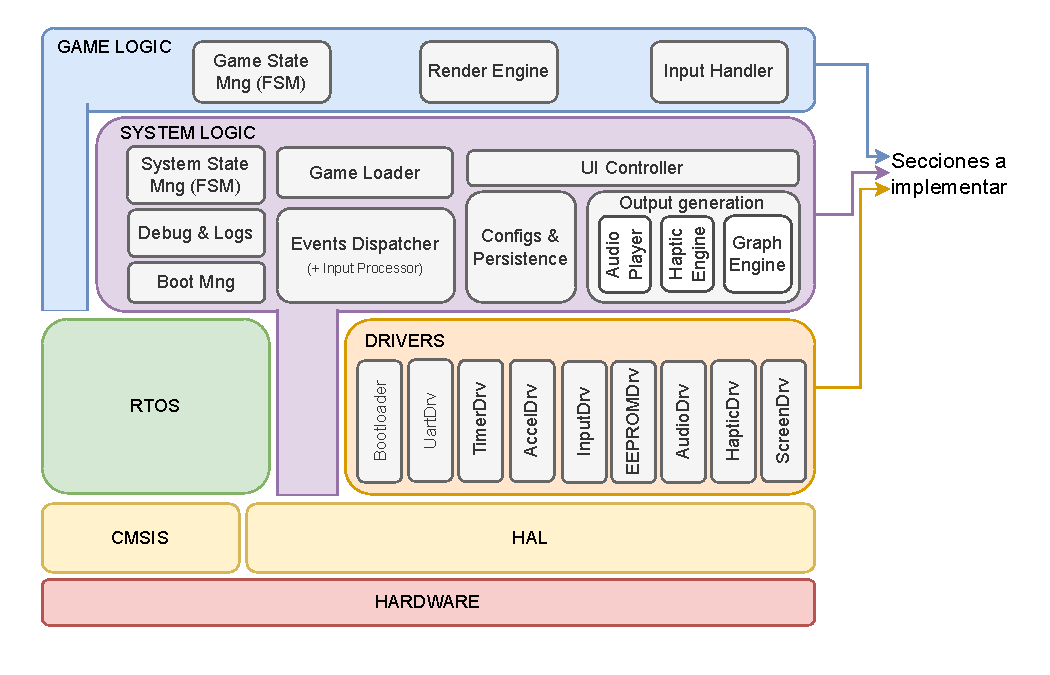
\includegraphics[width=.85\textwidth]{../Figuras/SW_layers.pdf}
\caption{Diagrama de capas del sistema.}
\label{fig:diagCapas}
\end{figure}


\subsection{Funciones del producto}
\label{sec:orgaf51da6}

\begin{enumerate}
  \item El software aquí especificado brindará las siguientes funcionalidades:
  \begin{enumerate}
    \item Gestión y procesamiento de las entradas mediante botones, joystick y acelerómetro.
    \item Gestión y generación de salidas de imagen, audio y vibración.
    \item Gestión de la persistencia del estado del juego en memoria no volátil.
    \item Gestión de partidas guardadas (selección, eliminación).
    \item Implementación de un demo de juego de simulación de vuelo en aeronave.
    \item Gestión de comunicaciones mediante UART para debug.
    \item Gestión y almacenamiento de logs para debug.
  \end{enumerate}
  \item El software aquí especificado no brindará los servicios de:
  \begin{enumerate}
    \item Conectividad externa con otros dispositivos más allá de los requeridos para programación del firmware y/o debug.
    \item Funcionalidades multijugador.
    \item Lectura o integración de otros juegos.
    \item Gestión o integración con periféricos diferentes a los mencionados en el documento RETRO\_GAME-RH-vA.
  \end{enumerate}
\end{enumerate}


\subsection{Características de los usuarios}
\label{sec:orga40b0ee}

\begin{enumerate}
  \item Los usuarios de este producto serán personas interesadas en consolas de juegos portátiles. 
  \item Se requiere la destreza básica para manejar botones, el joystick y la inclinación de la consola.
\end{enumerate}


\subsection{Restricciones}
\label{sec:org5ca5790}

\begin{enumerate}
  \item El software deberá mantenerse bajo control de versiones.
  \item El software deberá integrar apropiadamente los periféricos de entrada y salida descritos en el documento RETRO\_GAME-RH-vA.
\end{enumerate}


\subsection{Suposiciones y dependencias}
\label{sec:org0ae23fe}

\begin{enumerate}
  \item Se supone que se dispondrá de todos los componentes y de hardware a utilizar desde el comienzo de la fase de análisis hasta la finalización del desarrollo del software para la defensa pública.
\end{enumerate}


\subsection{Requisitos futuros}
\label{sec:org33cfcdb}

\begin{enumerate}
  \item Incorporación de funcionalidades de gestión de la energía, suspensión y/o lecturas del nivel de batería.
  \item Ampliación del demo de juego para incorporar nuevos eventos, desafíos o niveles.
  \item Incorporación de opciones de configuración (volumen de audio, brillo, intensidad de vibración).
\end{enumerate} 


\section{Requisitos específicos}
\label{sec:org40573d1}


\subsection{Interfaces externas}
\label{sec:orgfd5391f}

\begin{description}[labelindent=0.5cm]
  \item[\texttt{RETRO\_GAME-RS-REQ0001:}] el software deberá comunicarse por I2C con una memoria EEPROM.  
  \item[\texttt{RETRO\_GAME-RS-REQ0002:}] el software deberá comunicarse por SPI con una pantalla LED.
  \item[\texttt{RETRO\_GAME-RS-REQ0003:}] el software deberá comunicarse por I2C con un acelerómetro.
  \item[\texttt{RETRO\_GAME-RS-REQ0004:}] el software deberá generar una señal de audio mediante PWM hacia un amplificador externo.
  \item[\texttt{RETRO\_GAME-RS-REQ0005:}] el software deberá comunicarse por I2C con el módulo de vibración.
  \item[\texttt{RETRO\_GAME-RS-REQ0006:}] el software deberá adquirir entradas digitales mediante pines GPIO desde múltiples botones físicos.
  \item[\texttt{RETRO\_GAME-RS-REQ0007:}] el software deberá adquirir señales analógicas desde un joystick de dos ejes mediante entradas ADC.
  \item[\texttt{RETRO\_GAME-RS-REQ0008:}] el sistema deberá exponer, a través del conector USB del ST-Link de la placa, una interfaz UART para enviar logs de depuración a la PC. La consola de depuración deberá estar disponible en los estados \texttt{SYS\_SPLASH}, \texttt{SYS\_MAIN\_MENU}, \texttt{SYS\_IN\_GAME} y \texttt{SYS\_PAUSED}.
  \item[\texttt{RETRO\_GAME-RS-REQ0009:}] la consola de depuración deberá aceptar los comandos de texto «logon» y «logoff» para activar o silenciar la generación de trazas en tiempo de ejecución.
\end{description}


\subsection{Funciones}
\label{sec:org307bb59}

\subsubsection{Flujo de encendido}
\begin{description}[labelindent=0.5cm]
  \item[\texttt{RETRO\_GAME-RS-REQ0010:}] el sistema deberá entrar en estado \texttt{SYS\_SPLASH} dentro de los 250 ms posteriores al encendido o reset.
  \item[\texttt{RETRO\_GAME-RS-REQ0011:}] el sistema deberá permanecer en el estado \texttt{SYS\_SPLASH} durante no más de 1500 ms y luego pasar al estado \texttt{SYS\_MAIN\_MENU}, mostrando al menos las opciones «Iniciar nueva partida».
  \item[\texttt{RETRO\_GAME-RS-REQ0012:}] si se detecta una partida guardada válida, el estado \texttt{SYS\_MAIN\_MENU} deberá mostrar bajo la opción «Iniciar nueva partida» la aclaración de que se descartará la partida guardada.
  \item[\texttt{RETRO\_GAME-RS-REQ0013:}] si se detecta una partida guardada válida, el estado \texttt{SYS\_MAIN\_MENU} deberá mostrar además la opción «Continuar».
  \item[\texttt{RETRO\_GAME-RS-REQ0014:}] al seleccionar alguna de las opciones de inicio, se deberá pasar al estado \texttt{SYS\_IN\_GAME}.
  \item[\texttt{RETRO\_GAME-RS-REQ0015:}] al pasar a \texttt{SYS\_IN\_GAME} desde «Iniciar nueva partida», el sistema deberá descartar la partida guardada e iniciar una nueva partida.
  \item[\texttt{RETRO\_GAME-RS-REQ0016:}] al pasar a \texttt{SYS\_IN\_GAME} desde «Continuar», el sistema deberá cargar la partida guardada y restaurar el estado del juego antes de mostrar el primer fotograma.
\end{description}

\subsubsection{Flujo de pausa y opciones}
\begin{description}[labelindent=0.5cm]
  \item[\texttt{RETRO\_GAME-RS-REQ0017:}] al pulsar el botón START durante \texttt{SYS\_IN\_GAME}, el sistema deberá entrar en el estado \texttt{SYS\_PAUSED} en un tiempo no mayor a 500 ms y mostrar un menú con las opciones «Continuar», «Guardar» y «Salir».
  \item[\texttt{RETRO\_GAME-RS-REQ0018:}] mientras el sistema se encuentre en \texttt{SYS\_PAUSED}, el juego permanece detenido, no debe correr el tiempo ni modificar ninguna variable de estado.
  \item[\texttt{RETRO\_GAME-RS-REQ0019:}] al seleccionar «Continuar», el sistema deberá regresar al juego en el estado \texttt{SYS\_IN\_GAME} en un tiempo no mayor a 500 ms y reanudar todas las acciones detenidas.
  \item[\texttt{RETRO\_GAME-RS-REQ0020:}] al seleccionar «Guardar», el sistema deberá guardar la partida en la EEPROM en un tiempo no mayor a 500 ms, mostrar en pantalla el mensaje «Guardado exitoso» durante al menos 1000 ms y permanecer en \texttt{SYS\_PAUSED}.
  \item[\texttt{RETRO\_GAME-RS-REQ0021:}] si la operación de guardado falla, el sistema deberá mostrar «Error al guardar» durante al menos 1000 ms y permanecer en \texttt{SYS\_PAUSED}.
  \item[\texttt{RETRO\_GAME-RS-REQ0022:}] al seleccionar la opción «Salir», el sistema deberá descartar los cambios no guardados y pasar al estado \texttt{SYS\_MAIN\_MENU} en un tiempo no mayor a 1000 ms.
\end{description}

\subsubsection{Bucle de juego}
\begin{description}[labelindent=0.5cm]
  \item[\texttt{RETRO\_GAME-RS-REQ0023:}] el sistema deberá ejecutar el bucle de juego en el estado \texttt{SYS\_IN\_GAME} a una frecuencia mínima sostenida de 20\,FPS (período no mayor a 50 ms) bajo la carga típica del demo.
  \item[\texttt{RETRO\_GAME-RS-REQ0024:}] en cada cuadro, los eventos de entrada (botones, joystick, acelerómetro) deberán despacharse a la lógica del juego en un tiempo no mayor a 10 ms desde su captura por los drivers.
  \item[\texttt{RETRO\_GAME-RS-REQ0025:}] la lógica del juego deberá generar la lista de comandos de render y entregarla al driver de pantalla en un tiempo acumulado no mayor a 10 ms dentro del mismo cuadro.
  \item[\texttt{RETRO\_GAME-RS-REQ0026:}] cuando la lógica del juego solicite la reproducción de un efecto de sonido, el sistema deberá iniciar dicho efecto en la salida de audio en un tiempo no mayor a 10 ms.
  \item[\texttt{RETRO\_GAME-RS-REQ0027:}] cuando la lógica del juego dispare un evento de vibración, el sistema deberá activar el patrón de vibración correspondiente en un tiempo no mayor a 10 ms.
\end{description}


\subsection{Requisitos de rendimiento}
\label{sec:org94bc543}

\begin{description}[labelindent=0.5cm]
  \item[\texttt{RETRO\_GAME-RS-REQ0028:}] el sistema deberá mantener la frecuencia de cuadro dentro de ±5 \% de 20 FPS durante al menos el 95 \% del tiempo de ejecución continuo en \texttt{SYS\_IN\_GAME}.
\end{description}

\subsection{Restricciones de diseño}
\label{sec:org49fe900}

\begin{description}[labelindent=0.5cm]
  \item[\texttt{RETRO\_GAME-RS-REQ0029:}] el software deberá correr en la placa STM32 NUCLEO-F446RE.
  \item[\texttt{RETRO\_GAME-RS-REQ0030:}] se deberá utilizar el sistema operativo FreeRTOS para el manejo de las tareas del sistema.
\end{description}


\subsection{Atributos del sistema}
\label{sec:orgd0babc0}

N/A.

\subsection{Otros requisitos}
\label{sec:org31d2978}

N/A.

\newpage


\section{Apéndices}
\label{sec:org75cea03}

N/A.

\end{document}
